\section{Calibration and the gate}
\label{sec:calibration}

\subsection{Step and confirm}

Every run starts with a calibration of its own setpoints: each commanded platform voltage is
paired with what the line meter reads through the $\times$1000 divider. For each setpoint,
in order,
\begin{enumerate}
    \item the acquisition process writes the DAC and confirms the write;
    \item the meter waits for the point to settle, then takes \emph{one} reading on command;
    \item the reading is kept only if it was taken at least that long after its write;
        otherwise the reading (not the write) is asked for again after the shortfall.
\end{enumerate}
Reading $i$ cannot be asked for before write $i$ is confirmed, so setpoint and reading
cannot slip apart. Each reading integrates whole power line cycles
(\code{calibration: nplc}, 1 by default), which takes out the mains a short reading
catches. Retries are capped at three a point and ten a calibration; any other fault stops
the calibration with a sentence naming it.

\paragraph{Settling.}
SETTLE, 50\,ms, covers the amplifier's measured settling (a 2\,kV jump within 0.5\,V in
20.5\,ms). Where the \app{Settle time} page has measured a settle model, each jump waits
1.25 times its settling, if longer.

\subsection{The gate}

A \textbf{REJECT} writes no file and starts no scan; a \textbf{WARN} goes to the ELOG with
the run. The thresholds are \code{THRESHOLDS} in \code{cls\_acquisition/calibration.py},
and each run records those it was judged by.

\begin{center}
\begin{tabularx}{\textwidth}{@{}lL@{}}
\toprule
Check & Refuses (or warns) when \\
\midrule
length          & there is not one reading per planned setpoint \\
tracking        & the readback does not follow the command ($|r| < 0.90$) \\
span            & the readback's span is more than 10\,\% off the commanded span \\
polarity        & (WARN) the two converters' lines meet 0\,V more than 0.10\,V apart \\
settle          & a kept reading came sooner after its write than its jump takes to settle;
                  (WARN) setpoints were read again \\
held            & the last setpoint, read ten more times held 0.2\,s on, scatters over 0.5\,V,
                  or the calibration's last reading sits more than half a step (or six of
                  their scatter) from it: a lag of $k$ puts it $k$ steps off \\
plan            & the commanded voltages are not the plan, once each, in order \\
dac\_calibration & a measured DAC correction is past its validity; (WARN) one is in force,
                  since the bench table is applied after collection \\
\bottomrule
\end{tabularx}
\end{center}

\subsection{The Scan Calibration tab}

A calibration over any range, without a scan: set \app{From (V)}, \app{To (V)} and
\app{Stepsize (V)} and press \app{Start calibration}. The readback against setpoint, its
deviation and the measured step fill point by point; the gate's verdict and every check
follow (Figure~\ref{fig:calibration}). A scan's own calibration and an opened run's are
shown here too.

\paragraph{Against the bench table.}
With a bench table in force (Section~\ref{sec:table}), every calibration is fitted to it,
$V = a + b\,T$ at each point's DAC code, weighted by the meter's noise and the table's
10\,mV repeatability. The report gives $a$ (the run's 0\,V level), $b - 1$, the residual
against what those account for (WARN at twice that: the table is stale or the hardware
changed), how many points fell between the table's codes, and $a$ and $b$ of the last runs
on the same table. The fit is recorded with the run (\code{TableFit}); the header's
\code{CalSet} and \code{CalReadback} are unchanged.

\begin{figure}[ht]
    \centering
    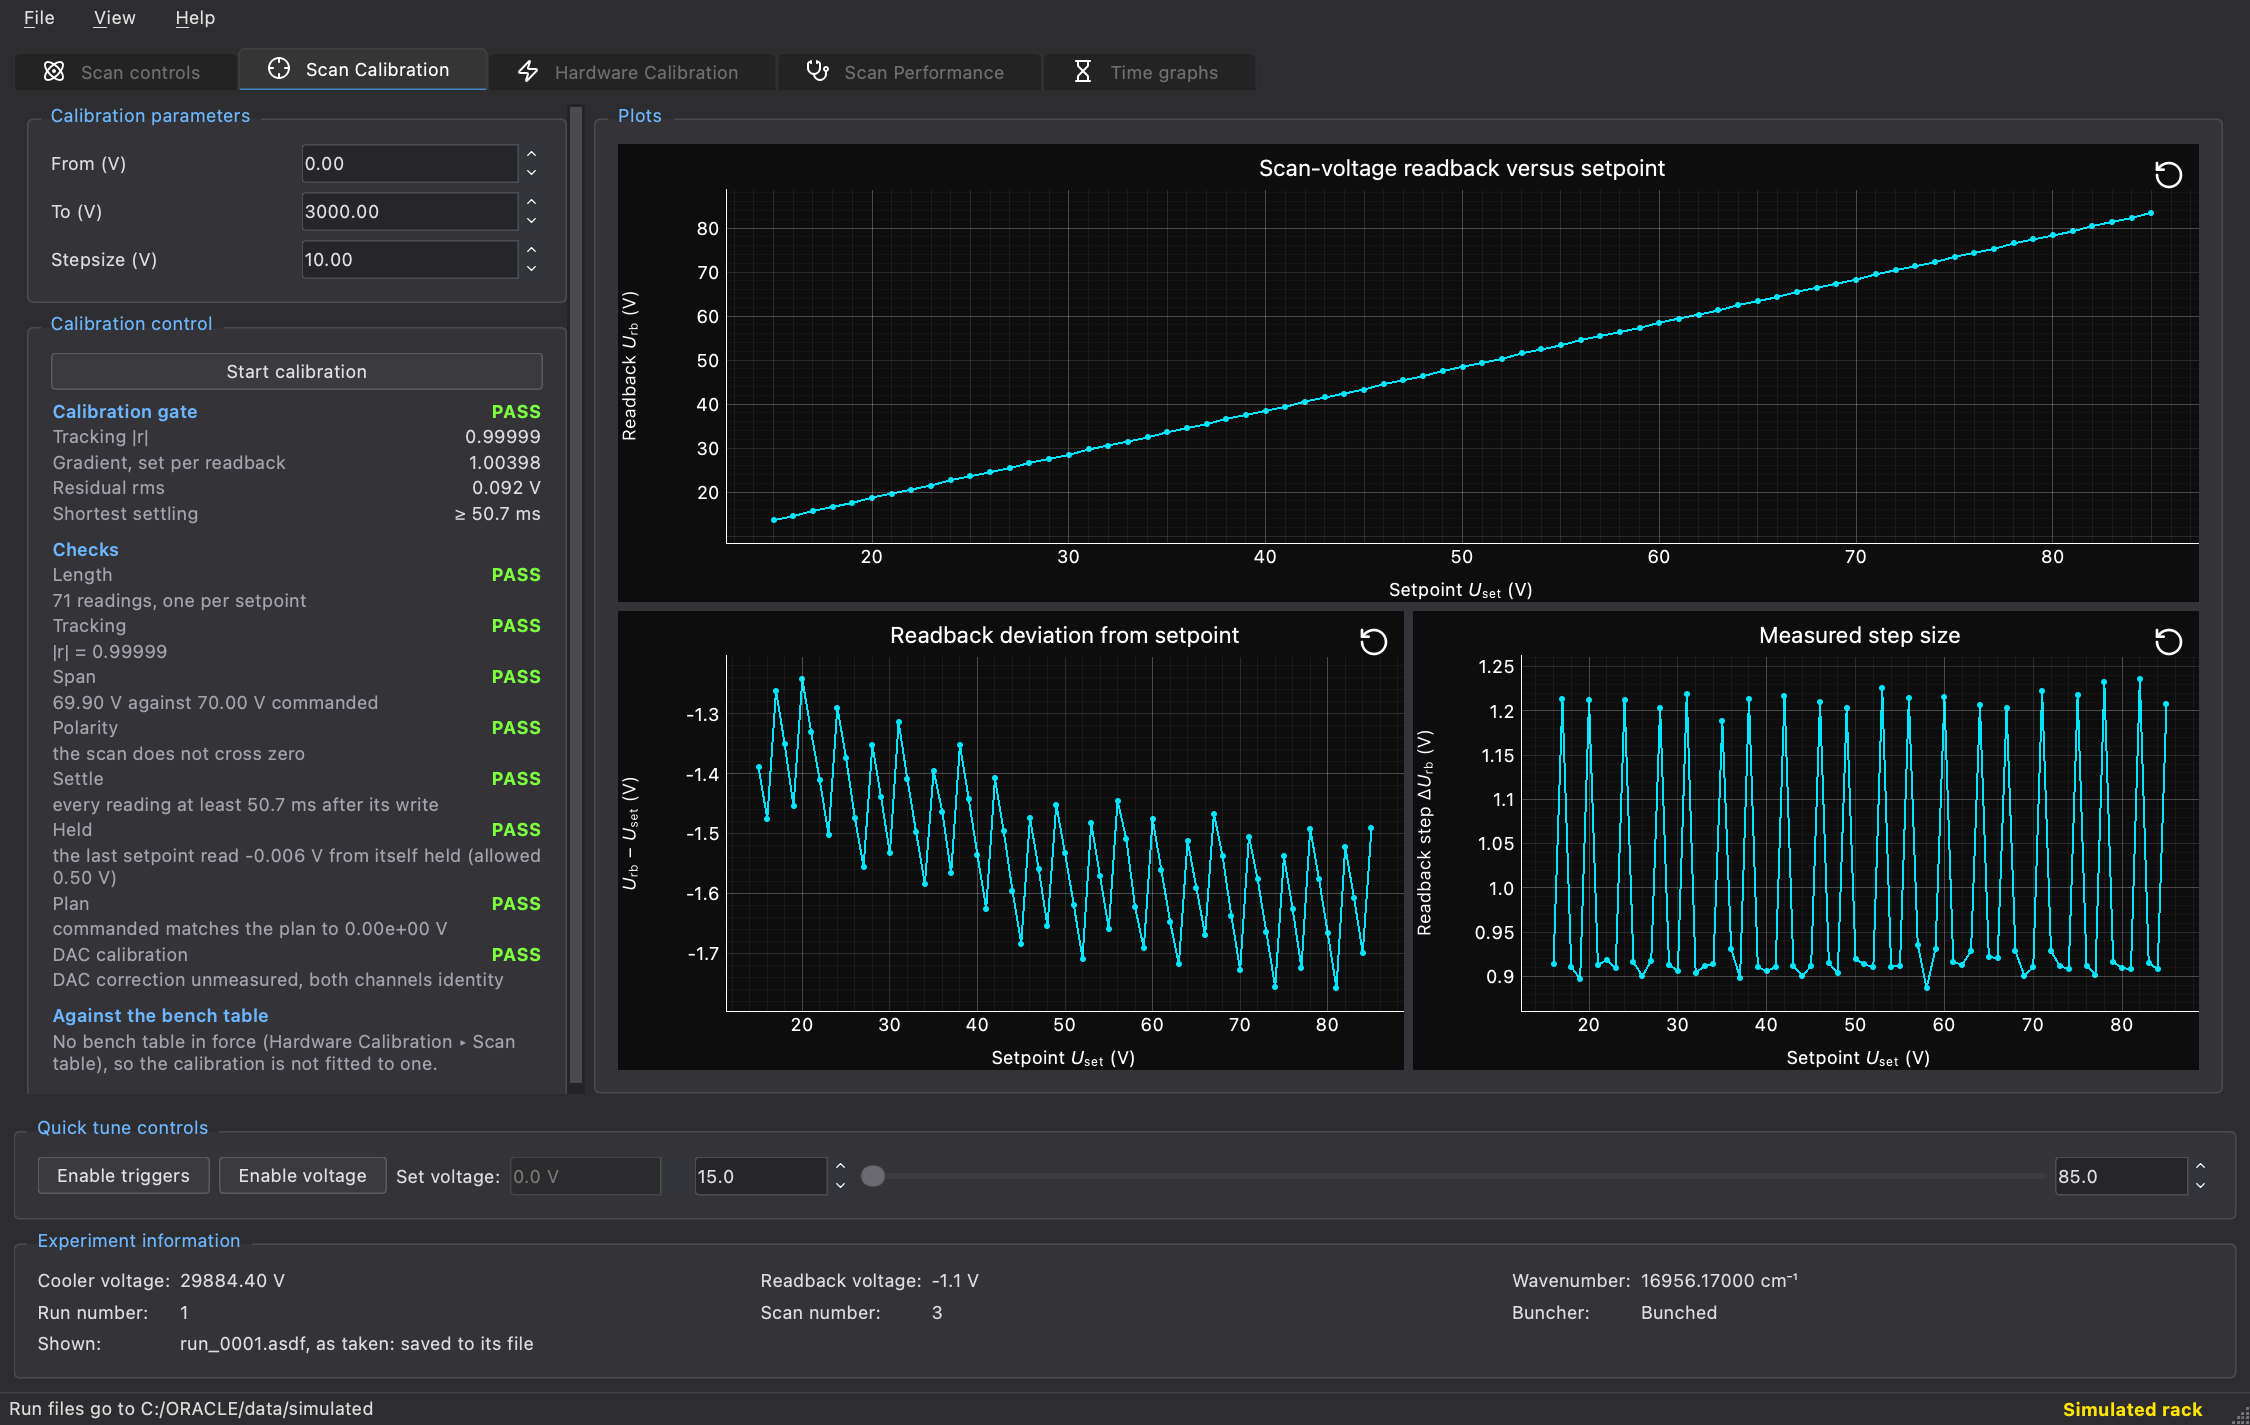
\includegraphics[width=\textwidth]{fig_calibration_tab}
    \caption{\app{Scan Calibration}: a run's calibration and the gate's report on it.}
    \label{fig:calibration}
\end{figure}
